\PassOptionsToPackage{unicode=true}{hyperref} % options for packages loaded elsewhere
\PassOptionsToPackage{hyphens}{url}
%
\documentclass[
]{article}
\usepackage{lmodern}
\usepackage{amssymb,amsmath}
\usepackage{ifxetex,ifluatex}
\ifnum 0\ifxetex 1\fi\ifluatex 1\fi=0 % if pdftex
  \usepackage[T1]{fontenc}
  \usepackage[utf8]{inputenc}
  \usepackage{textcomp} % provides euro and other symbols
\else % if luatex or xelatex
  \usepackage{unicode-math}
  \defaultfontfeatures{Scale=MatchLowercase}
  \defaultfontfeatures[\rmfamily]{Ligatures=TeX,Scale=1}
\fi
% use upquote if available, for straight quotes in verbatim environments
\IfFileExists{upquote.sty}{\usepackage{upquote}}{}
\IfFileExists{microtype.sty}{% use microtype if available
  \usepackage[]{microtype}
  \UseMicrotypeSet[protrusion]{basicmath} % disable protrusion for tt fonts
}{}
\makeatletter
\@ifundefined{KOMAClassName}{% if non-KOMA class
  \IfFileExists{parskip.sty}{%
    \usepackage{parskip}
  }{% else
    \setlength{\parindent}{0pt}
    \setlength{\parskip}{6pt plus 2pt minus 1pt}}
}{% if KOMA class
  \KOMAoptions{parskip=half}}
\makeatother
\usepackage{xcolor}
\IfFileExists{xurl.sty}{\usepackage{xurl}}{} % add URL line breaks if available
\IfFileExists{bookmark.sty}{\usepackage{bookmark}}{\usepackage{hyperref}}
\hypersetup{
  pdftitle={Tropical Cyclone Bibliography},
  pdfauthor={Matthew Hughes},
  pdfborder={0 0 0},
  breaklinks=true}
\urlstyle{same}  % don't use monospace font for urls
\usepackage[margin=1in]{geometry}
\usepackage{graphicx,grffile}
\makeatletter
\def\maxwidth{\ifdim\Gin@nat@width>\linewidth\linewidth\else\Gin@nat@width\fi}
\def\maxheight{\ifdim\Gin@nat@height>\textheight\textheight\else\Gin@nat@height\fi}
\makeatother
% Scale images if necessary, so that they will not overflow the page
% margins by default, and it is still possible to overwrite the defaults
% using explicit options in \includegraphics[width, height, ...]{}
\setkeys{Gin}{width=\maxwidth,height=\maxheight,keepaspectratio}
\setlength{\emergencystretch}{3em}  % prevent overfull lines
\providecommand{\tightlist}{%
  \setlength{\itemsep}{0pt}\setlength{\parskip}{0pt}}
\setcounter{secnumdepth}{-2}
% Redefines (sub)paragraphs to behave more like sections
\ifx\paragraph\undefined\else
  \let\oldparagraph\paragraph
  \renewcommand{\paragraph}[1]{\oldparagraph{#1}\mbox{}}
\fi
\ifx\subparagraph\undefined\else
  \let\oldsubparagraph\subparagraph
  \renewcommand{\subparagraph}[1]{\oldsubparagraph{#1}\mbox{}}
\fi

% set default figure placement to htbp
\makeatletter
\def\fps@figure{htbp}
\makeatother


\title{Tropical Cyclone Bibliography}
\author{Matthew Hughes}
\date{February 7, 2020}

\begin{document}
\maketitle

\hypertarget{kinney2008autism}{%
\section{(Kinney et al. 2008)}\label{kinney2008autism}}

\hypertarget{spatial-scale}{%
\subsection{Spatial Scale:}\label{spatial-scale}}

\begin{itemize}
\tightlist
\item
  ``National Weather Service maps of storm tracks were used to identify
  the parishes that were hit by the centers of each storm, and thus were
  likely to have experienced the most intense effects of the storm''
  (Kinney et al. 2008)
\end{itemize}

\hypertarget{exposure}{%
\subsection{Exposure:}\label{exposure}}

\begin{itemize}
\tightlist
\item
  Severity of prenatal storm exposure assessed two ways: intensity of
  storm's impact on parish, and how vulnerable residents would be if
  storm hit their parish. (Intensity and Vulnerability).
\item
  Using data from NCHS, 40 week gestations were assumed to estimate the
  gestional age of babies during the storm.
\end{itemize}

\hypertarget{resultsoutcomes}{%
\subsection{Results/Outcomes:}\label{resultsoutcomes}}

\begin{itemize}
\tightlist
\item
  AD(Autistic Disorder) had significantly higher prevalence in those
  with higher prenatal storm exposure. AD Prevalence also depended on
  Prenatal Period of Storm Exposure (what gestational period the baby
  was in when the storm exposure occured)
\end{itemize}

\hypertarget{bayleyegn2006rapid}{%
\section{(Bayleyegn et al. 2006)}\label{bayleyegn2006rapid}}

\hypertarget{spatial-scale-1}{%
\subsection{Spatial Scale:}\label{spatial-scale-1}}

\begin{itemize}
\tightlist
\item
  Escambia and Santa Rosa counties were identified as those most
  impacted by Hurricane Ivan by Florida Department of Health.
  Probability Proportional to Size Sampling (modified from the WHO), was
  used to obtain a sample of 30 clusters within these counties, which
  were put on maps given to interview teams.
\item
  7 households interviewed per cluster, for a total of 420 households
  interviewed.
\item
  Interviews administered asking for demographic info, housing info,
  damage info, etc.
\end{itemize}

\hypertarget{temporal-scale}{%
\subsection{Temporal scale}\label{temporal-scale}}

\begin{itemize}
\tightlist
\item
  Survey instruments administered over 3 days, 6 days after Hurricane
  Ivan made landfall.
\end{itemize}

\hypertarget{resultsoutcomes-1}{%
\subsection{Results/Outcomes}\label{resultsoutcomes-1}}

\begin{itemize}
\tightlist
\item
  Most commonly reported ``Greatest needs'' were garbage pickup and
  restoration of electricity, after that it was access to medical care,
  medications, home repair, and ice. -Interviews and surveys were
  intended to look at what the health and safety impacts were after the
  hurricane, it turned out to be a wide variety of factors including
  poor environmental hygiene, living in damaged homes, sleep
  disturbance, respiratory problems, and the aformentioned ``Greatest
  Needs.''
\end{itemize}

\hypertarget{hagy2006effects}{%
\section{(Hagy, Lehrter, and Murrell 2006)}\label{hagy2006effects}}

\hypertarget{temporalspatial-scale}{%
\subsection{Temporal/Spatial Scale:}\label{temporalspatial-scale}}

\begin{itemize}
\tightlist
\item
  Water quality surveys conducted monthly from 2000 to 2004 at up to 15
  sites located on two transects within the Pensacola Bay system. Post
  Hurricane Ivan surveys were taken October 6 and November 5, or 20 and
  50 days after the storm.\\
\item
  Extent of inundated land and maximum height of tidal surge were
  estimated by directly observing locations and heights of high water
  marks around perimeter of Pensacola Bay. -Total Prism Model used to
  estimate the magnitude of exchane associated with storm surge.
\end{itemize}

\hypertarget{outcomeresults}{%
\subsection{Outcome/Results:}\label{outcomeresults}}

\begin{itemize}
\tightlist
\item
  Hurricane Ivan caused water to rise continuously for 31 hours.
\item
  Storm surge inundated 165 km\^{}2 of land, which increased the Bay's
  surface area by 50\% and it's volume by 230\%.
\item
  Based on Total Prism Model, storm surge flushed a maximum of 60\% of
  the Bay's water out to sea as it retreated - this must have increased
  salinity of the Bay substantially.
\item
  Using Navy's model estimate of offshore salinity in the Tidal Prism
  Model, Ivan's surge was computed to have increased the mean salinity
  of the Bay from 23.4 to as high as 30.0.
\item
  Tidal surge replaced Bay waters with low-nutrient, well-oxygenated,
  oligotrophic Gulf waters
\item
  Post-storm freshwater input stimulated an increase in phytoplankton
  biomass, which persisted for several weeks.
\item
  Hypoxia was intensified relative to the seasonal norm.
\end{itemize}

\hypertarget{lieberman2017self}{%
\section{(Lieberman-Cribbin et al. 2017)}\label{lieberman2017self}}

\hypertarget{spatial-scale-2}{%
\subsection{Spatial Scale:}\label{spatial-scale-2}}

\begin{itemize}
\tightlist
\item
  Self reported flood data
\item
  ``Public macro-level flood data was obtained from the FEMA Modeling
  Task Force (MOTF) Hurricane Sandy Impact Analysis'' (Lieberman-Cribbin
  et al. 2017)
\item
  New York State 3 meter spatial resolution storm surge product
  downloaded and imported into licensed version of ArcGIS to provide
  water depth above ground in New York City and Long Island
\item
  Street level geo-coding in SAS using datasets generated from U.S.
  Census Bureau TIGER/Line shapefiles. Process matches street, city, and
  zip-code from survey dataset with lookup dataset to produce a
  coordinate
\end{itemize}

\hypertarget{resultsoutcomes-2}{%
\subsection{Results/Outcomes:}\label{resultsoutcomes-2}}

\begin{itemize}
\tightlist
\item
  Mental health variables considered based on scores of a questionaire
  were anxiety score, depression score, and PTSD score
\item
  Self reported flood exposure and FEMA flood exposure data showed
  significant discrepencies in the associations between flooding and
  mental health outcomes.
\item
  Self reported dichotomous flooding showed significant associations
  with all mental health outcomes, whereas dichotomous FEMA flooding
  only showed significant associations with PTSD.
\item
  Macro-level flooding data is less expensive and faster, but
  potentially underestimates mental health outcomes.
\end{itemize}

\hypertarget{grabich2016hurricane}{%
\section{(S. C. Grabich et al. 2016)}\label{grabich2016hurricane}}

\hypertarget{spatial-scale-3}{%
\subsection{Spatial Scale:}\label{spatial-scale-3}}

\begin{itemize}
\tightlist
\item
  Births to (only) Florida residents linked to address to link to
  hurricane exposure
\item
  Hurricane risk assessed at county level
\item
  Florida Department of Health, Vital Statistics Department was the
  source of data on births from 2003 to 2005.
\item
  Hurricane exposure classified as maximum wind speed in specific
  Florida county extracted from NOAA's Hurricane Research Division
  public database.
\item
  Exposure defined as \textgreater{}= 39 mph and \textgreater{}= 74 mph
\end{itemize}

\hypertarget{temporal-scale-1}{%
\section{Temporal Scale:}\label{temporal-scale-1}}

\begin{itemize}
\tightlist
\item
  Risk period begins at 20 weeks of gestation
\item
  Pregnancy divided into exposed time and unexposed time after 20 weeks
\item
  Study population included births with estimated date of conception
  between October 24, 2003 and September 26, 2004.
\end{itemize}

\hypertarget{resultsoutcomes-3}{%
\section{Results/Outcomes}\label{resultsoutcomes-3}}

\begin{itemize}
\item
  Outcome of interest was to see if there was an association between
  hurricane exposure and the risk of a preterm birth.
\item
  Two outcome standards: extremely preterm delivery \textless{} 32 weeks
  gestation, and overall preterm delivery \textless{} 37 weeks
  gestation.
\item
  Overall positive association observed between exposure to Hurricane
  Harvey and hazard of extreme preterm delivery (not overall preterm
  delivery however)
\item
\end{itemize}

\hypertarget{scaramutti2019mental}{%
\section{(Scaramutti et al. 2019)}\label{scaramutti2019mental}}

\hypertarget{spatial-scale-4}{%
\subsection{Spatial Scale:}\label{spatial-scale-4}}

\begin{itemize}
\tightlist
\item
  Major cities in Florida and Puerto Rico were coded as urban with 0,
  and all other areas were coded as rural/suburban with a 1.
\item
  Word of mouth and outreach to community leaders and community centers
  in Central and South Florida and Puerto Rico
\item
  Online surveys available through Qualtrics, respondants asked to refer
  3 additional respondants
\item
  Linear regression models used with site and urbanacity as predictors
  for depressive symptoms, anxiety symptoms, and PTSD symptoms
\item
  Binary logistic regression analysis for clinical vs non-clinical
  anxiety, depression, and PTSD as criterion variables, and site or
  urbanacity as predictors
\end{itemize}

\hypertarget{temporal-scale-2}{%
\subsection{Temporal Scale:}\label{temporal-scale-2}}

\begin{itemize}
\tightlist
\item
  Assessing mental health of Puerto Ricans in Florida and Puerto Rico 6
  months after Hurricane Maria.
\end{itemize}

\hypertarget{resultsoutcomes-4}{%
\subsection{Results/Outcomes:}\label{resultsoutcomes-4}}

\begin{itemize}
\tightlist
\item
  Mental health outcomes of interest were anxiety, depression, and PTSD
\item
  Results showed significant associations between urbanacity and
  anxiety, approaching statistical significance for association between
  urbanacity and depressive symptoms, and significant association
  between urbanacity and PTSD intrusive reexperiencing and PTSD
  hypervigilance.
\item
  Overall, rates of depression and PTSD were higher in Puerto Ricans who
  migrated to Florida after Hurricane Maria.
\item
  Puerto Ricans outside major cities were more likely to meet criteria
  for depression and PTSD
\item
  Puerto Ricans in Puerto Rico had significantly fewere clinical
  symptoms than those in Florida, but rates were high overall for both
  Florida and Puerto Rico.
\end{itemize}

\hypertarget{bianchette2009ecological}{%
\section{(Bianchette et al. 2009)}\label{bianchette2009ecological}}

\hypertarget{temporalspatial-scale-1}{%
\subsection{Temporal/Spatial Scale:}\label{temporalspatial-scale-1}}

\begin{itemize}
\tightlist
\item
  Study area was three coastal lakes known as the Shelby Lakes in Gulf
  State Park, Alabama.
\item
  Hurrican Ivan brought 120 mph winds and a storm surge of 10-12 feet,
  which inundated all of the coastal plane around the Shelby Lakes.
\item
  Post hurricane images of vegetation take 9.5 months after hurricane to
  ensure that vegetation damage observed was permanent.
\item
  Remote sensing using Landsat 5 images coupled with ground surveys of
  tree mortality were used.
\end{itemize}

\hypertarget{resultsoutcomes-5}{%
\subsection{Results/Outcomes:}\label{resultsoutcomes-5}}

\begin{itemize}
\tightlist
\item
  Ecological impacts were the main concern of this study, primarily
  measured by tree mortality.
\item
  Trees at lower elevation showed greater mortality than those at higher
  elevations.
\item
  Results suggested that saltwater intrusion and storm surge flooding
  were the main reasons for tree mortality in forests around Shelby
  Lakes, rather than wind damage.
\end{itemize}

\hypertarget{grabich2016measuring}{%
\section{(S. Grabich et al. 2016)}\label{grabich2016measuring}}

\hypertarget{spatialtemporal-scale}{%
\subsection{Spatial/Temporal Scale:}\label{spatialtemporal-scale}}

\begin{itemize}
\tightlist
\item
  Hurricane disaster exposure 3 methods, FEMA Presidential disaster
  declarations, spatial data on specific storm trajectory (storm tracks
  with a symmmetrical buffer around them), novel meteorological measure
  based on Saffir-Simpson hurricane intensity scale.
\item
  Preterm birth and low birth weight rates collected from the county
  level of exposed areas
\end{itemize}

\hypertarget{bevilacqua2020understanding}{%
\section{(Bevilacqua et al. 2020)}\label{bevilacqua2020understanding}}

\hypertarget{spatial-scale-5}{%
\subsection{Spatial Scale}\label{spatial-scale-5}}

\begin{itemize}
\tightlist
\item
  ggmaps package in R was used to generate distribution of zip codes of
  the participants
\end{itemize}

\hypertarget{temporal-scale-3}{%
\subsection{Temporal Scale}\label{temporal-scale-3}}

\hypertarget{lane2013health}{%
\section{(Lane et al. 2013)}\label{lane2013health}}

\hypertarget{spatial-scale-6}{%
\subsection{Spatial Scale}\label{spatial-scale-6}}

\begin{itemize}
\tightlist
\item
  ``Based on vulnerable subgroups identified in the literature,
  potential indicators of population vulnerability for which data are
  available were identified and mapped within the 42 NYC United Hospital
  Fund (UHF) neighborhoods located within any NYC hurricane evacuation
  zone. UHF neighborhoods are zip code-aggregated areas within all five
  boroughs. For each indicator, prevalences were categorized
  intoquartilesbyneighborhood.''
\end{itemize}

\hypertarget{lane2013health-1}{%
\section{(Lane et al. 2013)}\label{lane2013health-1}}

\hypertarget{schwartz2018preliminary}{%
\section{(Schwartz et al. 2018)}\label{schwartz2018preliminary}}

\hypertarget{spatial}{%
\subsection{Spatial}\label{spatial}}

\begin{itemize}
\tightlist
\item
  Convenience sampling from the Greater Houston area
\end{itemize}

\hypertarget{temporal}{%
\subsection{Temporal}\label{temporal}}

\begin{itemize}
\tightlist
\item
  Research team arrived in Houston less than 3 weeks after Hurricane
  Harvey made landfall
\end{itemize}

\hypertarget{pugatch2019tropical}{%
\section{(Pugatch 2019)}\label{pugatch2019tropical}}

\begin{itemize}
\tightlist
\item
  ``I use windspeed data on tropical storms originating in the Atlantic
  and eastern North Pacific oceans (the regions relevant to Mexico),
  available from the National Oceanic and Atmospheric Administration
  (NOAA) Tropical Prediction Center, a U.S. government agency. NOAA
  analyzes data from reconnaissance aircraft, ships, and satellites to
  create ``best tracks'' of individual storms: positions (latitude and
  longitude) of storm centers at 6-hourly intervals, combined with
  intensity information (windspeed and barometric pressure; Jarvinen,
  Neumann, \& Davis, 1993; Davis, Brown, \& Preston, 1984; Chu, Sampson,
  Levine, \& Fukada, 2002). Complete records for both ocean regions are
  available since 1949. Fig. 1 maps storm best tracks making landfall in
  Mexico" (Pugatch 2019)
\item
  ``I use data on tropical storm exposure and mortality in all 31
  Mexican states, plus Mexico City, for each month during 1990-- 2011 (I
  chose the starting period based on the availability of microdata on
  mortality). I create an index to measure storm severity by
  incorporating two elements, windspeed and population density''
  ({\textbf{???}})
\end{itemize}

\hypertarget{jaycox2010children}{%
\section{(Jaycox et al. 2010)}\label{jaycox2010children}}

New Orleans schoolchildren were participated in a trial and assessment
of an intervention after Hurricane Katrina. Group intervention at school
and individual intervention at a clinic were the two options. Both
treatments led to a reduction in symptoms of PTSD, but there were still
elevated levels of PTSD even post treatment.

\hypertarget{spatial-scale-7}{%
\subsection{Spatial Scale}\label{spatial-scale-7}}

\begin{itemize}
\tightlist
\item
  Three schools in New Orleans participating in Project Fleur-de-Lis.
\end{itemize}

\hypertarget{temporal-scale-4}{%
\subsection{Temporal Scale}\label{temporal-scale-4}}

\begin{itemize}
\tightlist
\item
  Interventions began 15 months after Hurricane Katrina.
\item
  "Students were assessed at baseline (December 2006--January 2007), at
  5 months (April--May 2007) and at 10 months (September--October 2007).
  The CBITS groups ran March to May 2007 and TF-CBT was implemented
  February to September,
\end{itemize}

\begin{enumerate}
\def\labelenumi{\arabic{enumi}.}
\setcounter{enumi}{2006}
\tightlist
\item
  This study only reports on the 10-month follow-up assessment
  results."(Jaycox et al. 2010)
\end{enumerate}

\hypertarget{exposure-1}{%
\subsection{Exposure}\label{exposure-1}}

\begin{itemize}
\tightlist
\item
  Exposure measured via self report by students using the Disaster
  Experience Questionnaire.
\item
  ``For an overall exposure to hurricane experiences measure, we tallied
  experiences listed in the top panel of Table 2, for a total number of
  experiences per student.'' (Jaycox et al. 2010)
\item
  PTSD symptoms assessed using the Child PTSD Symptom Scale (a score
  greater than 11 is considered elevated symptoms).
\end{itemize}

\hypertarget{resultsoutcomes-6}{%
\subsection{Results/Outcomes}\label{resultsoutcomes-6}}

\begin{itemize}
\tightlist
\item
  More girls than boys were at risk for PTSD symptoms (63\% for girls,
  and 37\% for boys).
\item
  PTSD scores at 10 months were generally improved from scores at
  baseline assessment in students who participated in the intervention.
\item
  ``More than 60\% of students screened positive for elevated PTSD
  symptoms and were included in the intervention field trial.'' (Jaycox
  et al. 2010)
\end{itemize}

\hypertarget{bourque2006weathering}{%
\section{(Bourque et al. 2006)}\label{bourque2006weathering}}

\hypertarget{temporal-scale-5}{%
\subsection{Temporal Scale}\label{temporal-scale-5}}

\hypertarget{spatial-scale-8}{%
\subsection{Spatial Scale}\label{spatial-scale-8}}

\hypertarget{exposure-2}{%
\subsection{Exposure}\label{exposure-2}}

\hypertarget{resultsoutcomes-7}{%
\subsection{Results/Outcomes}\label{resultsoutcomes-7}}

\begin{itemize}
\tightlist
\item
  NOAA's Tropical Prediction Center estimates that between 1970 and
  1999, 1\% of deaths in hurricanes were caused by storm surges, 59\% by
  freshwater (inland) flooding, and 12\% by wind.
\end{itemize}

\hypertarget{harville2010population}{%
\section{(Harville et al. 2010)}\label{harville2010population}}

\begin{itemize}
\tightlist
\item
  Low birth rates and preterm births were studied in Louisiana at three
  spatial levels: Orleans Parish (New Orleans), Region 1 (this includes
  Orleans Parish, and several others), and Louisiana as a whole.
\end{itemize}

\hypertarget{temporal-scale-6}{%
\subsection{Temporal Scale}\label{temporal-scale-6}}

\begin{itemize}
\tightlist
\item
  Data used in analysis came from Louisiana birth records 2003-2007, in
  Medicaid-linked data.
\item
  Birth outcomes among state residents were examined for the 2 years
  before and after Hurricane Katrina.
\end{itemize}

\hypertarget{spatial-scale-9}{%
\subsection{Spatial Scale}\label{spatial-scale-9}}

\begin{itemize}
\tightlist
\item
  The Regional Level is the scale that was used to study birth outcomes,
  and Louisiana is divided into 9 health regions.
\item
  The Region of mother's residence was used to study rather than the
  region that the mother gave birth in.
\item
  Region 1 was the Louisiana region hit most strongly by Hurricane
  Katrina and consists of Orleans,Jefferson,Plaquemines,and St Bernard
  parishes. The study looked at Orleans parish (city of New Orleans),
  Region 1, and Louisiana all together.
\end{itemize}

\hypertarget{exposure-3}{%
\subsection{Exposure}\label{exposure-3}}

\begin{itemize}
\tightlist
\item
  Exposure defined as giving birth in the two years after Hurricane
  Katrina
\end{itemize}

\hypertarget{resultsoutcome}{%
\subsection{Results/Outcome}\label{resultsoutcome}}

\begin{itemize}
\tightlist
\item
  Outcomes of interest were Low Birth Weight, and Preterm Birth.
\item
  In Louisiana as a whole, rates of LBW rose in the two years after
  Hurricane Katrina, but rates of Preterm births did not.
\item
  Overall, Hurricane Katrina was not associated with an increase in the
  rates of LBW and preterm births, in some areas there was a reduction
  of these. This may be due to population changes though because the
  population at risk after the hurricane had a higher risk profile.
\end{itemize}

\hypertarget{ferdinand2005hurricane}{%
\section{(Ferdinand 2005)}\label{ferdinand2005hurricane}}

\begin{itemize}
\tightlist
\item
  Hurricane Katrina led to a large number of people with uncontrolled
  hypertension and cardiovascular disease. Higher rates of high blood
  pressure are seen in African Americans than in whites, and the rates
  of controlled blood pressure in disadvantaged communities in Louisiana
  is very low.
\end{itemize}

\hypertarget{spatial-scale-10}{%
\subsection{Spatial Scale}\label{spatial-scale-10}}

\begin{itemize}
\tightlist
\item
  680 adults staying in Hurricane Katrina shelters in Houston Texas were
  given a survey
\item
  98\% of these survey subjects were from New Orleans.
\item
  Population in areas of flooding was 76\% black, and 29\% below the
  poverty line.
\end{itemize}

\hypertarget{temporal-scale-7}{%
\subsection{Temporal Scale}\label{temporal-scale-7}}

\begin{itemize}
\tightlist
\item
  Surveys were administered from September 10 - 12, 2005.
\end{itemize}

\hypertarget{exposure-4}{%
\subsection{Exposure}\label{exposure-4}}

\begin{itemize}
\tightlist
\item
  Exposure to flooding leads to evacuation and unexpected displacement,
  which increases the odds of losing medical records and information
  that include hypertensive patient's medication regimen, including
  frequency, dosage, and indications.
\end{itemize}

\hypertarget{resultsoutcome-1}{%
\subsection{Results/Outcome}\label{resultsoutcome-1}}

\begin{itemize}
\tightlist
\item
  Outcomes of concern in this paper are hypertension and cardiovascular
  disease.
\item
  ``There is a 1.8x greater rate of fatal stroke, 1.5x greater rate of
  coronary heart disease and mortality, and a 4.2x greater rate of
  end‐stage renal disease in this population.'' (Ferdinand 2005)
\item
  ``Only 52\% of evacuees had health insurance at the time of the
  hurricane, and chronic conditions such as heart disease, hypertension,
  diabetes, and asthma were reported by 41\% of the adults surveyed.
  Furthermore, 29\% of evacuees reported having problems in obtaining
  their necessary prescription drugs.'' (Ferdinand 2005)
\end{itemize}

\hypertarget{christopher2017effects}{%
\section{(Christopher 2017)}\label{christopher2017effects}}

\hypertarget{temporal-scale-8}{%
\subsection{Temporal Scale}\label{temporal-scale-8}}

\begin{itemize}
\tightlist
\item
  July 1, 2004 to August 31, 2006 for Hurricane Katrina.
\item
  March 1, 2010 to April 31, 2012 for April 2011 Alabama tornado
  disaster.
\item
  ``The gestation period for mothers in the sample ranged from 18 to 47
  weeks, with a mean gestation period of 37.97 weeks (SD = 2.84
  weeks''{[}christopher2017effects{]}
\end{itemize}

\hypertarget{spatial-scale-11}{%
\subsection{Spatial Scale}\label{spatial-scale-11}}

\begin{itemize}
\tightlist
\item
  ``For Hurricane Katrina, the population was delimited to pregnant
  women residing in the counties of Hancock, Harrison, Jackson, and
  Jones, Mississippi, who experienced a live singleton birth which
  survived or was born and died between the periods of July 1, 2004 to
  August 31, 2006.'' (Christopher 2017)
\item
  ``For the April 2011 Alabama tornado disaster, the population was
  delimited to pregnant women residing in the counties of Calhoun,
  DeKalb, Franklin, Jefferson, Lawrence, Limestone, Madison, Marion,
  St.~Clair, and Tuscaloosa, Alabama who were most likely affected by
  the April 2011 tornado disaster, and experienced a live singleton
  birth which survived or was born and died between the periods of March
  1, 2010 to April 31, 2012.'' (Christopher 2017)
\end{itemize}

\hypertarget{exposure-5}{%
\subsection{Exposure}\label{exposure-5}}

\begin{itemize}
\tightlist
\item
  Maternal prenatal exposure to Hurricane Katrina in Mississippi
\item
  Maternal prenatal exposure to April 2011 Tornado disaster in Alabama.
\item
  ``The data consisted of customized delimited county-level linked birth
  and infant death data drawn from Alabama and Mississippi Linked Infant
  Births and Deaths Record Files for the period 1997-2013.''
  (Christopher 2017)
\end{itemize}

\hypertarget{resultsoutcome-2}{%
\subsection{Results/Outcome}\label{resultsoutcome-2}}

\begin{itemize}
\tightlist
\item
  Response variables of interest included birth weight, preterm birth,
  infant mortality, and mode of delivery.
\item
  Exposure to hurricanes increased odds of low birth weight and also
  increased risk for preterm birth, however it wasn't shown to have a
  significant association with increased infant mortality.
\end{itemize}

\begin{figure}

{\centering 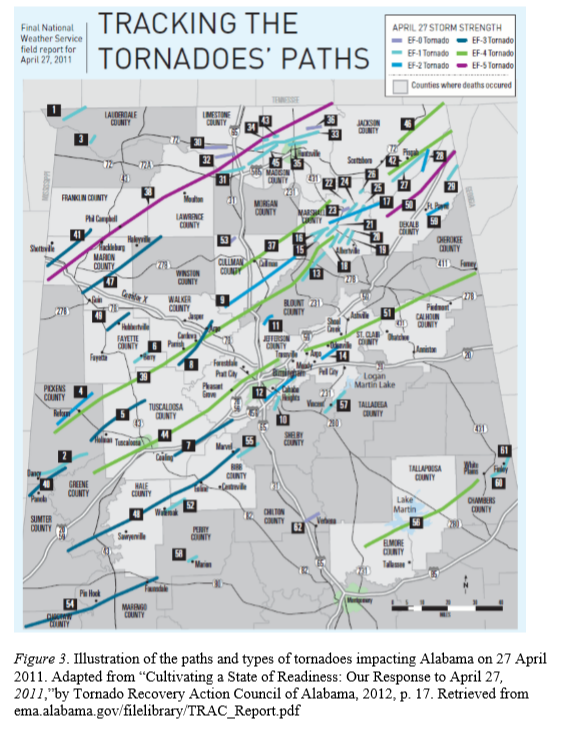
\includegraphics[width=0.4\textwidth]{figures/Tracking_The_Tornadoes_Paths_in_Alabama} 

}

\caption{Example of how exposure to tornadoes was assesses in Christopher (2017) for counties.}\label{fig:unnamed-chunk-1}
\end{figure}

\begin{figure}

{\centering 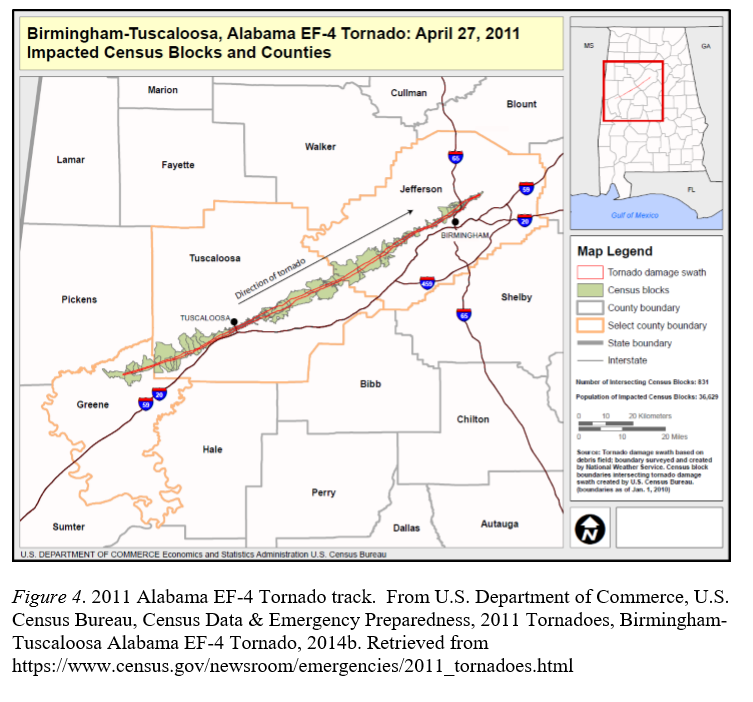
\includegraphics[width=0.4\textwidth]{figures/Birmingham_Tuscaloosa_Tornado_Track} 

}

\caption{Second Figure.}\label{fig:unnamed-chunk-2}
\end{figure}

\hypertarget{zahran2011economics}{%
\section{(Zahran et al. 2011)}\label{zahran2011economics}}

\hypertarget{temporal-scale-9}{%
\subsection{Temporal Scale}\label{temporal-scale-9}}

\begin{itemize}
\tightlist
\item
  ``Mental health condition is measured as the reported count of poor
  mental health days experienced by a respondent in the previous 30
  days. Data on mental health days are from the CDC's BRFSS,
  2005--2006.'' (Zahran et al. 2011)
\end{itemize}

\hypertarget{spatial-scale-12}{%
\subsection{Spatial Scale}\label{spatial-scale-12}}

\begin{itemize}
\item
  Intensity of hurricane's path measured using data on property damage
  and crop loss from the Spatial Hazard Losses and Events Database.
\item
\end{itemize}

\hypertarget{exposure-6}{%
\subsection{Exposure}\label{exposure-6}}

\begin{itemize}
\tightlist
\item
  ``Individual exposure to Hurricane Katrina and/or Rita was determined
  by information on the temporal and spatial coordinates of each
  hurricane event, the date a respondent was interviewed by the CDC, and
  the respondent's place of county residence, as reported in the CDC's
  Behavioral Risk Factor Surveillance System (BRFSS) database'' (Zahran
  et al. 2011)
\item
  Number of poor mental healthd days expected to have spikes
  corresponding to hurricane events in affected but not unaffected areas
  with respect to hurricane exposure.
\end{itemize}

\hypertarget{resultsoutcomes-8}{%
\subsection{Results/Outcomes}\label{resultsoutcomes-8}}

\begin{itemize}
\tightlist
\item
  Outcome of interest was mental health resilience of Hurricane Katrina
  and Rita survivors, stratified by vulnerability status. Number of poor
  mental health days used as metric for this.
\item
  Vulnerability status measured by poor physical health, social support,
  education level, income, and being a single mother.
\item
  Single mothers were identified as a particular vulnerability category
  of interest
\item
  ``Resistance refers to the capacity to limit displacement from
  equilibrium following a traumatic event. Resilience, by contrast,
  points to the ability to return to an equilibrium state---the more
  rapid the return to preevent functioning, the greater the
  resilience.'' (Zahran et al. 2011)
\item
  Average number of poor mental health days in 30 was 3.37 for the
  population as a whole, and 5.95 for single mothers.
\item
  Overall, hurricane exposed single mothers and exposed ``others'' all
  experienced an increased number of days of poor mental health.
\item
  ``We estimate that single mothers, as a group, suffered over \$130
  million in productivity loss from added postdisaster stress and
  disability.'' (Zahran et al. 2011)
\end{itemize}

(Zahran, Tavani, and Weiler 2013)

\hypertarget{temporal-scale-10}{%
\subsection{Temporal Scale}\label{temporal-scale-10}}

\hypertarget{spatial-scale-13}{%
\subsection{Spatial Scale}\label{spatial-scale-13}}

\begin{itemize}
\item
  Casualty counts are recorded at the county level in counties affected
  by either hurricanes or tornados.
\item
\end{itemize}

\hypertarget{exposure-7}{%
\subsection{Exposure}\label{exposure-7}}

\begin{itemize}
\tightlist
\item
  ``In the event of a natural disaster,people living in affected areas
  suffer both income and wealth losses. Wealth losses typically involve
  damage to residential or commercial property, whereas income losses
  involve lost wages, profits, dividends, and rents in consequence of the
  disaster.'' (Zahran, Tavani, and Weiler 2013)
\end{itemize}

\hypertarget{resultsoutcomes-9}{%
\subsection{Results/Outcomes}\label{resultsoutcomes-9}}

\begin{itemize}
\tightlist
\item
  Dependent variables analyzed are hurricane casualties and tornado
  casualties.
\item
  Predictor variables are disaster damage, recency bias, and day of the
  week.
\end{itemize}

\hypertarget{references}{%
\section*{References}\label{references}}
\addcontentsline{toc}{section}{References}

\hypertarget{refs}{}
\leavevmode\hypertarget{ref-bayleyegn2006rapid}{}%
Bayleyegn, Tesfaye, Amy Wolkin, Kathleen Oberst, Stacy Young, Carlos
Sanchez, Annette Phelps, Joann Schulte, Carol Rubin, and Dahna Batts.
2006. ``Rapid Assessment of the Needs and Health Status in Santa Rosa
and Escambia Counties, Florida, After Hurricane Ivan, September 2004.''
\emph{Disaster Management \& Response} 4 (1): 12--18.

\leavevmode\hypertarget{ref-bevilacqua2020understanding}{}%
Bevilacqua, Kristin, Rehana Rasul, Samantha Schneider, Maria Guzman,
Vishnu Nepal, Deborah Banerjee, Joann Schulte, and Rebecca M Schwartz.
2020. ``Understanding Associations Between Hurricane Harvey Exposure and
Mental Health Symptoms Among Greater Houston-Area Residents.''
\emph{Disaster Medicine and Public Health Preparedness}, 1--8.

\leavevmode\hypertarget{ref-bianchette2009ecological}{}%
Bianchette, TA, K-B Liu, NS-N Lam, and LM Kiage. 2009. ``Ecological
Impacts of Hurricane Ivan on the Gulf Coast of Alabama: A Remote Sensing
Study.'' \emph{Journal of Coastal Research}, 1622--6.

\leavevmode\hypertarget{ref-bourque2006weathering}{}%
Bourque, Linda B, Judith M Siegel, Megumi Kano, and Michele M Wood.
2006. ``Weathering the Storm: The Impact of Hurricanes on Physical and
Mental Health.'' \emph{The Annals of the American Academy of Political
and Social Science} 604 (1): 129--51.

\leavevmode\hypertarget{ref-christopher2017effects}{}%
Christopher, Kenneth E. 2017. ``The Effects of Hurricane and Tornado
Disasters on Pregnancy Outcomes.'' PhD thesis, Walden University.

\leavevmode\hypertarget{ref-ferdinand2005hurricane}{}%
Ferdinand, Keith C. 2005. ``The Hurricane Katrina Disaster: Focus on the
Hypertensive Patient.'' \emph{The Journal of Clinical Hypertension} 7
(11): 679--80.

\leavevmode\hypertarget{ref-grabich2016measuring}{}%
Grabich, SC, J Horney, C Konrad, and DT Lobdell. 2016. ``Measuring the
Storm: Methods of Quantifying Hurricane Exposure with Pregnancy
Outcomes.'' \emph{Natural Hazards Review} 17 (1): 06015002.

\leavevmode\hypertarget{ref-grabich2016hurricane}{}%
Grabich, Shannon C, Whitney R Robinson, Stephanie M Engel, Charles E
Konrad, David B Richardson, and Jennifer A Horney. 2016. ``Hurricane
Charley Exposure and Hazard of Preterm Delivery, Florida 2004.''
\emph{Maternal and Child Health Journal} 20 (12): 2474--82.

\leavevmode\hypertarget{ref-hagy2006effects}{}%
Hagy, James D, John C Lehrter, and Michael C Murrell. 2006. ``Effects of
Hurricane Ivan on Water Quality in Pensacola Bay, Florida.''
\emph{Estuaries and Coasts} 29 (6): 919--25.

\leavevmode\hypertarget{ref-harville2010population}{}%
Harville, Emily W, Tri Tran, Xu Xiong, and Pierre Buekens. 2010.
``Population Changes, Racial/Ethnic Disparities, and Birth Outcomes in
Louisiana After Hurricane Katrina.'' \emph{Disaster Medicine and Public
Health Preparedness} 4 (S1): S39--S45.

\leavevmode\hypertarget{ref-jaycox2010children}{}%
Jaycox, Lisa H, Judith A Cohen, Anthony P Mannarino, Douglas W Walker,
Audra K Langley, Kate L Gegenheimer, Molly Scott, and Matthias Schonlau.
2010. ``Children's Mental Health Care Following Hurricane Katrina: A
Field Trial of Trauma-Focused Psychotherapies.'' \emph{Journal of
Traumatic Stress: Official Publication of the International Society for
Traumatic Stress Studies} 23 (2): 223--31.

\leavevmode\hypertarget{ref-kinney2008autism}{}%
Kinney, Dennis K, Andrea M Miller, David J Crowley, Emerald Huang, and
Erika Gerber. 2008. ``Autism Prevalence Following Prenatal Exposure to
Hurricanes and Tropical Storms in Louisiana.'' \emph{Journal of Autism
and Developmental Disorders} 38 (3): 481--88.

\leavevmode\hypertarget{ref-lane2013health}{}%
Lane, Kathryn, Kizzy Charles-Guzman, Katherine Wheeler, Zaynah Abid,
Nathan Graber, and Thomas Matte. 2013. ``Health Effects of Coastal
Storms and Flooding in Urban Areas: A Review and Vulnerability
Assessment.'' \emph{Journal of Environmental and Public Health} 2013.

\leavevmode\hypertarget{ref-lieberman2017self}{}%
Lieberman-Cribbin, Wil, Bian Liu, Samantha Schneider, Rebecca Schwartz,
and Emanuela Taioli. 2017. ``Self-Reported and Fema Flood Exposure
Assessment After Hurricane Sandy: Association with Mental Health
Outcomes.'' \emph{PLoS One} 12 (1): e0170965.

\leavevmode\hypertarget{ref-pugatch2019tropical}{}%
Pugatch, Todd. 2019. ``Tropical Storms and Mortality Under Climate
Change.'' \emph{World Development} 117: 172--82.

\leavevmode\hypertarget{ref-scaramutti2019mental}{}%
Scaramutti, Carolina, Christopher P Salas-Wright, Saskia R Vos, and Seth
J Schwartz. 2019. ``The Mental Health Impact of Hurricane Maria on
Puerto Ricans in Puerto Rico and Florida.'' \emph{Disaster Medicine and
Public Health Preparedness} 13 (1): 24--27.

\leavevmode\hypertarget{ref-schwartz2018preliminary}{}%
Schwartz, Rebecca M, Stephanie Tuminello, Samantha M Kerath, Janelle
Rios, Wil Lieberman-Cribbin, and Emanuela Taioli. 2018. ``Preliminary
Assessment of Hurricane Harvey Exposures and Mental Health Impact.''
\emph{International Journal of Environmental Research and Public Health}
15 (5): 974.

\leavevmode\hypertarget{ref-zahran2011economics}{}%
Zahran, Sammy, Lori Peek, Jeffrey G Snodgrass, Stephan Weiler, and Lynn
Hempel. 2011. ``Economics of Disaster Risk, Social Vulnerability, and
Mental Health Resilience.'' \emph{Risk Analysis: An International
Journal} 31 (7): 1107--19.

\leavevmode\hypertarget{ref-zahran2013daily}{}%
Zahran, Sammy, Daniele Tavani, and Stephan Weiler. 2013. ``Daily
Variation in Natural Disaster Casualties: Information Flows, Safety, and
Opportunity Costs in Tornado Versus Hurricane Strikes.'' \emph{Risk
Analysis} 33 (7): 1265--80.

\end{document}
